\documentclass{beamer}

\usepackage[english]{babel}
\usepackage{amsmath,amsthm,amsfonts}
\usepackage{xkeyval}
\usepackage{graphics}
\usepackage{float}
\usepackage{url}
\usepackage{colortbl}%color a table
\usepackage[lined,boxed,linesnumbered]{algorithm2e}
\usepackage{CJKutf8}

\definecolor{mycolor}{RGB}{0,255,0}
\definecolor{mycolorlys}{RGB}{173,255,47}
\definecolor{mycolorlyslys}{RGB}{127,255,0}
\definecolor{mycolorlyslyslys}{RGB}{124,252,0}

\definecolor{rowcolor1}{RGB}{132,112,255}
\definecolor{rowcolor2}{RGB}{135,206,250}
\definecolor{rowcolor3}{RGB}{255,245,238}
\definecolor{colcolor1}{RGB}{255,165,0}
\definecolor{colcolor2}{RGB}{255,20,147}
\definecolor{colcolor3}{RGB}{147,112,219}

%输入罗马数字
\newcommand{\myRoman}[1]{\uppercase\expandafter{\romannumeral#1}}
\newcommand{\myroman}[1]{\romannumeral#1}

\mode<presentation>
{
	\usetheme{Madrid}
	\usecolortheme[named=mycolor]{structure}
	\useinnertheme{rectangles}
	\useoutertheme{infolines}%default,infolines,miniframes,shadow,sidebar,smoothbars,smoothtree,split,tree
	\usefonttheme[onlymath]{serif}
	\setbeamercovered{transparent}
	\setbeamertemplate{blocks}[rounded][shadow=true]
	\setbeamertemplate{background}{
\includegraphics[height=\paperheight,width=\paperwidth]{images/backgrounds}}%设置背景图片
}

\title{Report on UFLDL-Part \myRoman{2}}
\author{Yunfei WANG}
\institute{\inst{1}School of Computer Science \& Technology \\ Huazhong University of Science \& Technology}
\date{June 18th, 2013}
%\logo{
\includegraphics[scale=0.07]{images/HUSTLogo}}

\begin{document}
\begin{CJK*}{UTF8}{gbsn}

\begin{frame}
\titlepage
\end{frame}

\begin{frame}\frametitle{Table of contents}
\tableofcontents
\end{frame}

\section{Softmax Regression}
\subsection{Logistic Regression}
\begin{frame}\frametitle{Logistic Regression-Binary Classification}
\begin{columns}
\begin{column}{0.45\linewidth}
\centering
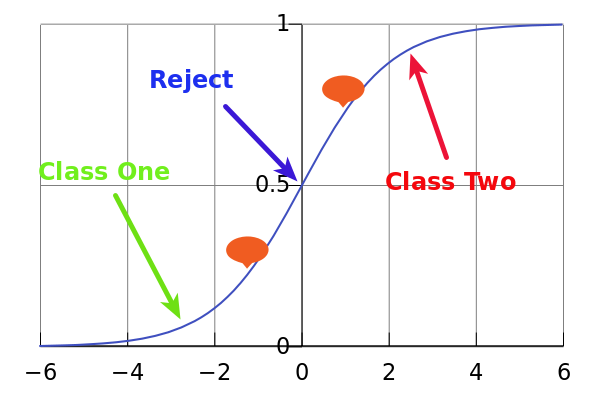
\includegraphics[scale=0.25]{images/sigmoidfun}
\end{column}
\begin{column}{0.6\linewidth}
\centering
\begin{equation}
h_{\theta}(x)=\frac{1}{1+\exp(-\theta^Tx)}\propto \exp(\theta^Tx)
\end{equation}
\end{column}
\end{columns}
Training set $\{(x^1,y^1),(x^2,y^2),\cdots,(x^m,y^m)|x^i\in\Re^{n+1},y^i\in\{0,1\}\}$.\\
\vspace{1cm}
Train the model parameters $\theta$ to minimize the following cost function:
\begin{equation}
J(\theta)=-\frac{1}{m}\left[\sum_{i=1}^my^i\log h_\theta(x^i)+(1-y^i)\log(1-h_{\theta}(x^i))\right]
\end{equation}
\end{frame}

\subsection{Generalize Logistic Regression to Softmax Regression}
\begin{frame}\frametitle{Generalize Logistic Regression to Softmax Regression}
\begin{figure}
\centering
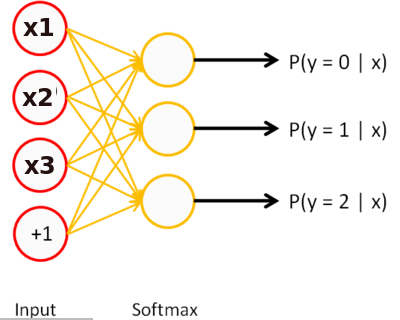
\includegraphics[scale=0.25]{images/Softmax_Classifier}
\end{figure}
Training set $\{(x^1,y^1),(x^2,y^2),\cdots,(x^m,y^m)|x^i\in\Re^{n+1},y^i\in\{1,\cdots,k\}\}$.\\
Estimate the probability for each class:
\begin{equation}\label{eq:softmax_output}
h_\theta(x^i)=\left[\begin{array}{c}
p(y^i=1|x;\theta)\\
p(y^i=2|x;\theta)\\
\vdots\\
p(y^i=k|x;\theta)\\
\end{array}\right]
=\frac{1}{\sum_{j=1}^k\exp(\theta_j^Tx^i)}\left[\begin{array}{c}
\exp(\theta_1^Tx^i)\\
\exp(\theta_2^Tx^i)\\
\vdots\\
\exp(\theta_k^Tx^i)
\end{array}\right]
\end{equation}
where $\theta_1,\theta_2,\cdots,\theta_k\in\Re^{n+1}$ are parameters of model,$\theta$ is a matrix obtained by stacking up $\theta_1,\theta_2,\cdots,\theta_k$ in rows.
\end{frame}

\subsection{Cost Function}
\begin{frame}[allowframebreaks]\frametitle{Cost Function}
Cost Function used for softmax regression:
\begin{equation}
J(\theta)=-\frac{1}{m}\left[\sum_{i=1}^m\sum_{j=1}^k1\{y^i=j\}\log\frac{\exp(\theta_j^Tx^i)}{\sum_{l=1}^k\exp(\theta_l^Tx^i)}\right]
\end{equation}
where $1\{\cdot\}$ is \textcolor{blue}{indicator function}:$1\{True\}=1,1\{False\}=0$.\\
\vspace{0.5cm}
Taking partial derivatives,we get the following gradient:
\begin{equation}\label{eq:pthetaj}
\nabla_{\theta_j}J(\theta)=-\frac{1}{m}\sum_{i=1}^m\left[x^i(1\{y^i=j\}-p(y^i=j|x^i;\theta))\right]
\end{equation}
Armed with the derivative,algorithm such as gradient descent an L-BFGS can be used to minimize $J(\theta)$.\\

\newpage
Next,make a brief derivation for the gradient above.Considering a single sample $(x^i,y^i)$:
\begin{itemize}
\item when $y^i=j$:
\begin{equation}
J(\theta;x^i)=\sum_{j=1}^k1\{y^i=j\}\log\frac{\exp(\theta_j^Tx^i)}{\sum_{l=1}^k\exp(\theta_l^Tx^i)}=\log\frac{\exp(\theta_j^Tx^i)}{\sum_{l=1}^k\exp(\theta_l^Tx^i)}
\end{equation}
\begin{equation}
\nabla_{\theta_j}J(\theta;x^i)=x^i(1-p(y^i=j|x^i;\theta))
\end{equation}
\item when $y^i=t\neq j$:
\begin{equation}
J(\theta;x^i)=\sum_{j=1}^k1\{y^i=j\}\log\frac{\exp(\theta_j^Tx^i)}{\sum_{l=1}^k\exp(\theta_l^Tx^i)}=\log\frac{\exp(\theta_t^Tx^i)}{\sum_{l=1}^k\exp(\theta_l^Tx^i)}
\end{equation}
\begin{equation}
\nabla_{\theta_j}J(\theta;x^i)=x^i(0-p(y^i=j|x^i;\theta))
\end{equation}
\end{itemize}
\end{frame}

\subsection{Properties of softmax regression parameterization}
\begin{frame}\frametitle{Properties of softmax regression parameterization}
Softmax regression has a \textcolor{blue}{"redundant"} set of parameters:
\begin{equation}
\begin{split}
p(y^i=j|x^i;\theta)=&\frac{\exp((\theta_j-\psi)^Tx^i)}{\sum_{l=1}^k\exp((\theta_l-\psi)^Tx^i)}\\
&=\frac{\exp(\theta_j^Tx^i)\exp(-\psi^Tx^i)}{\sum_{l=1}^k\exp(\theta_l^Tx^i)\exp(-\psi^Tx^i)}\\
&=\frac{\exp(\theta_j^Tx^i)}{\sum_{l=1}^k\exp(\theta_l^Tx^i)}
\end{split}
\end{equation}
In other words,subtracting $\psi$ from every $\theta_j$ doesn't affect predictions at all.\\
\begin{itemize}
\item By setting $\psi=\theta_1$,we could eliminate one parameter $\theta_1$
\item Preprocessing inner product to avoid overflow when computing $\exp(\theta_l^Tx^i)$
\end{itemize}
\end{frame}

\subsection{Weight Decay}
\begin{frame}\frametitle{Weight Decay}
Add weight decay term to penalize large values of parameters.\\
Our cost function is now:
\begin{equation}
J(\theta)=-\frac{1}{m}\left[\sum_{i=1}^m\sum_{j=1}^k1\{y^i=j\}\log\frac{\exp(\theta_j^Tx^i)}{\sum_{l=1}^k\exp(\theta_l^Tx^i)}\right]+\frac{\lambda}{2}\sum_{i=1}^k\sum_{j=1}^n\theta_{ij}^2
\end{equation}
With weight decay term(for any $\lambda\geq 0$),the cost function $J(\theta)$ is strictly convex and is guaranteed to have a unique solution.\\
To apply an optimization algorithm,compute its derivative:
\begin{equation}
\nabla_{\theta_j}J(\theta)=-\frac{1}{m}\sum_{i=1}^m\left[x^i(1\{y^i=j\}-p(y^i=j|x^i;\theta))\right]+\lambda\theta_j
\end{equation}
Because $J(\theta)$ is convex,algorithms such as gradient descent and L-BFGS are guaranteed to converge to global minimum.
\end{frame}

\subsection{Softmax Regression vs. Logistic Regression}
\begin{frame}\frametitle{Softmax Regression vs. Logistic Regression}
For multi-class classification application,which one is more suitable?\\
\vspace{1cm}
\begin{columns}
\begin{column}{0.5\linewidth}
Mutually exclusive classes
\begin{itemize}
\item indoor\_scene
\item outdoor\_urban\_scene
\item outdoor\_wilderness\_scene
\end{itemize}
\textcolor{blue}{Softmax regression is appropriate in this situation.}
\end{column}
\begin{column}{0.5\linewidth}
Classes not mutually exclusive
\begin{itemize}
\item pop music
\item dance music
\item vocal music
\end{itemize}
\textcolor{cyan}{Building separate logistic regression classifiers.}
\end{column}
\end{columns}
\end{frame}

\begin{frame}\frametitle{Experiments on Softmax/Logistic Regression}
\begin{table}
\begin{tabular}{|c|c|c|}
\rowcolor{rowcolor1}
Dataset & Dimensionality & Number of Samples\\
\rowcolor{rowcolor2}
Training Data & $784$ & $60000$\\
\rowcolor{rowcolor3}
Testing Data & $784$ & $10000$\\
\end{tabular}
\caption{MNIST}
\end{table}

\begin{table}
\begin{tabular}{|>{\columncolor{colcolor1}}c|>{\columncolor{colcolor2}}c|>{\columncolor{colcolor3}}c|}
\hline
 Classifier & Accuracy & Time Consumed\\
 \hline
 Softmax Regression & $92.63\%$ & $352$sec\\
 \hline
 Logistic Regression & $81.84\%$ & $218$sec\\
 \hline
\end{tabular}
\caption{Experiments Results}
\end{table}
\end{frame}

\section{Linear Decoders with Autoencoders}
\begin{frame}\frametitle{Linear Decoders with Autoencoders}
\begin{columns}
\begin{column}{0.35\linewidth}
\begin{figure}
\centering
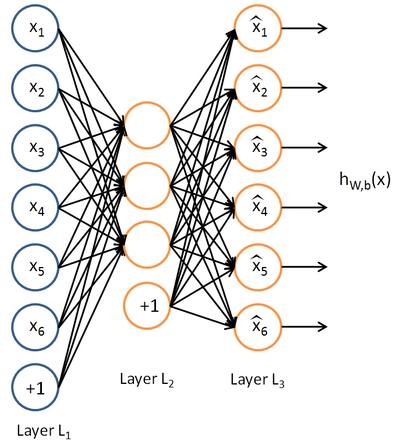
\includegraphics[scale=0.15]{images/Autoencoder}
\caption{Autoencoder}
\end{figure}
\end{column}
\begin{column}{0.7\linewidth}
Each neuron in output layer compute the following:
\begin{equation}
z^3=W^2a^2+b^2
\end{equation}
\begin{equation}
\hat{x}=a^3=f(z^3)
\end{equation}\\
\vspace{20pt}
\textcolor{magenta}{Limitation}:Input must be scaled in the range $[0,1]$.
\end{column}
\end{columns}
\textcolor{blue}{Linear decoder}:modify the activation function of output layer into an identity one,leaving the others unchanged.
\begin{equation}
\hat{x}=a^3=z^3=W^2a^2+b^2
\end{equation}
\textcolor{red}{Advantage}:Real-valued inputs without pre-scale can be processed!\\
We only need to change the error terms of output layer:
\begin{equation}
\delta_i^3=\frac{\partial}{\partial z_i}\frac{1}{2}\|y-\hat{x}\|^2=(\hat{x}_i-y_i)\cdot f'(z_i^3)=(\hat{x}_i-y_i)
\end{equation}
\end{frame}

\begin{frame}\frametitle{Experiments on Linear Decoder}
Dataset:$100,000$ small $8\times 8$ patches sampled from STL-10 color images.
\begin{columns}
\begin{column}{0.5\linewidth}
\begin{figure}
\centering
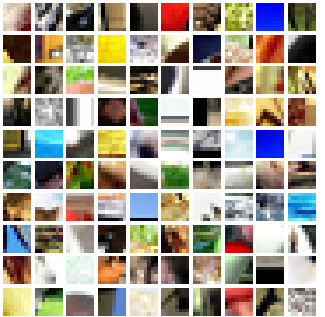
\includegraphics[scale=0.18]{images/STL10_Samples}
\caption{Training Samples}
\end{figure}
\end{column}
\begin{column}{0.5\linewidth}
\begin{figure}
\centering
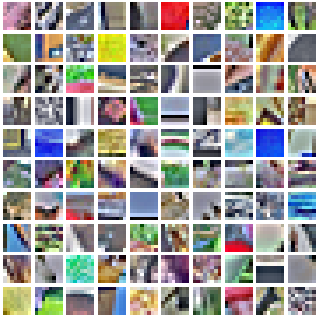
\includegraphics[scale=0.18]{images/STL10_PCAWhiten}
\caption{PCA-Whitened Samples}
\end{figure}
\end{column}
\end{columns}
\begin{figure}
\centering
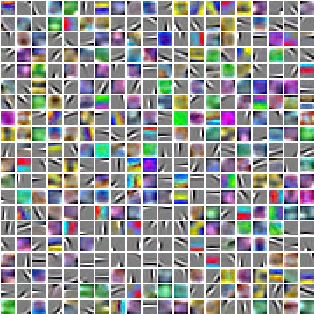
\includegraphics[scale=0.27]{images/weightsSTL10_60k}
\caption{Learned Features(Time Consumed:$2305$sec)}
\end{figure}

\end{frame}

\section{Self-Taught Learning}
\begin{frame}\frametitle{Self-Taught Learning}
\textcolor{magenta}{An aphorism in machine learning,"sometimes it's not who has the best algorithm than wins;it's who has the most data."}\\
\vspace{10pt}
\textcolor{blue}{Self-Taught Learning}:exploit massive unlabeled data effectively to learn good feature representations of input.\\
\vspace{10pt}
For classification task,we will combine feature representations extracted from labeled data and their labels to train a classifier.\\
\begin{alertblock}{Self-Taught Learning and Semi-Supervised Learning}
\begin{itemize}
\item \emph{Self-Taught Learning}\\
Unlabeled and labeled data may come from different distributions.
\item \emph{Semi-Supervised Learning}\\
Unlabeled and labeled data comes from exactly the same distribution.
\end{itemize}
\end{alertblock}
Apparently,Self-Taught Learning is more broadly applicable.
\end{frame}

\begin{frame}\frametitle{Learning Features}
\begin{columns}
\begin{column}{0.5\linewidth}
Train a sparse autoencoder on unlabeled data to get parameters $W^1,b^1,W^2,b^2$:
\begin{figure}
\centering
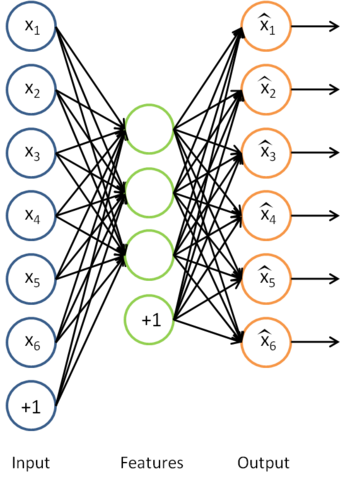
\includegraphics[scale=0.5]{images/STL_SparseAE}
\end{figure}
\end{column}
\begin{column}{0.5\linewidth}
Given any input $x$,compute the corresponding vector of activations $a$ of hidden units:
\begin{figure}
\centering
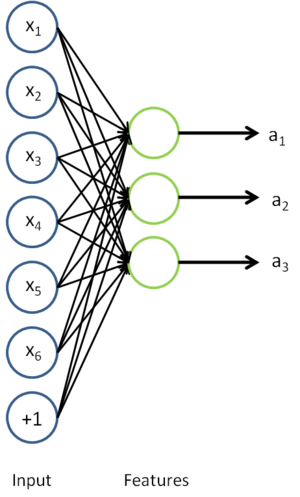
\includegraphics[scale=0.5]{images/STL_SparseAE_Features}
\end{figure}
\end{column}
\end{columns}
Next,for a labeled sample $(x_l,y_l)$,we can use $(a_l,y_l)$ or $((x_l,a_l),y_l)$ to represent it.
\end{frame}

\begin{frame}\frametitle{Experiments on Self-Taught Learning}
\begin{center}
\textcolor{red}{Learned Features}+\textcolor{purple}{Softmax Classifier}
\end{center}
\begin{table}
\begin{tabular}{|c|c|c|}
\hline
Dataset & Dimensionality & Number of Samples\\
\rowcolor{rowcolor1}
Unlabeled Data($5\sim 10$) & $784$ & $29404$\\
\rowcolor{rowcolor2}
Training Data($0\sim 4$) & $784$ & $15298$\\
\rowcolor{rowcolor3}
Testing Data($0\sim 4$) & $784$ & $15298$\\
\end{tabular}
\end{table}
\begin{figure}
\centering
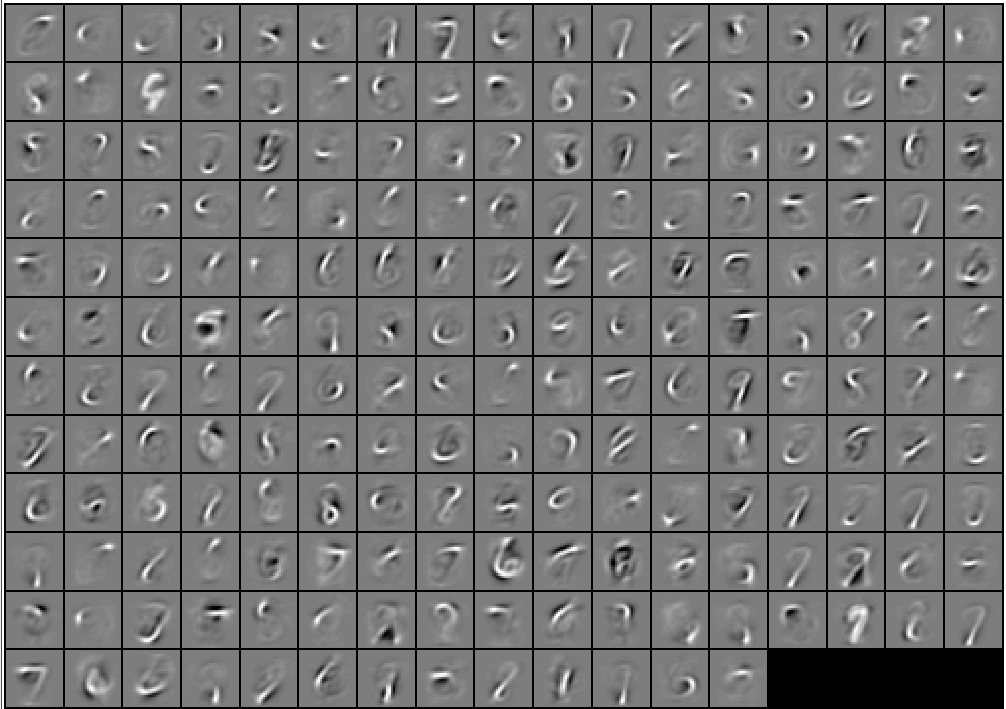
\includegraphics[scale=0.1]{images/MNIST_weights}
\caption{Learned Features on unlabeled data}
\end{figure}
\begin{center}
Accuray:$98.3\%$,Time Consumed:$6064$sec
\end{center}
\end{frame}

\end{CJK*}
\end{document}
